\section{Sprache}\label{sec:language}

Kern dieses Abschnitts ist eine neue Beschreibungssprache für textuelle Beispielszenarien.
Diese trägt den Namen Scenario-Sprache.
Ziel der Scenario-Sprache ist es, verständlich für jeden zu sein, der Englisch spricht.
Um als Programmiersprache funktionsfähig zu sein, hat sie im Gegensatz zu Englisch eine feste und eingeschränkte grammatikalische Struktur.
Somit handelt es sich um eine Untermenge der Englischen Sprache.
Des Weiteren basiert die Scenario-Sprache auf dem Markdown-Format,
das es erlaubt, einfachen Text mit Überschriften, Fett- und Kursivschreibung, Bildern u.ä.\ zu versehen.
Markdown-Dateien können leicht in HTML umgewandelt werden,
wodurch in der Scenario-Sprache verfasste Texte auch als Dokumentation einsetzbar sind.
Im Folgenden werden einige Grundlagen der Scenario-Sprache dargestellt und erklärt.

\subsection{Grundlagen}\label{subsec:basics}

\begin{listing}[htp]
    \begin{minipage}{0.45\textwidth}
        \centering
        \inputminted{md}{chapter/fulib-scenarios/scenarios/Basic.md}
        \captionof{listing}{Basic.md}
    \end{minipage}
    \hspace{0.05\textwidth}
    \begin{minipage}{0.45\textwidth}
        \centering
        \inputminted{java}{chapter/fulib-scenarios/java/BasicTest.java}
        \captionof{listing}{BasicTest.java}
    \end{minipage}
    \caption{Beispiel für Grundlagen der Scenario-Sprache}
    \label{lst:basic-example}
\end{listing}

In der Scenario-Sprache verfasster Quellcode wird in \code{.md}-Dateien abgelegt.
Listing~\ref{lst:basic-example} zeigt links ein Beispiel für eine solche.
Rechts davon ist der Java-Code zu sehen, der zu dieser Datei äquivalent ist.

Eine Scenario-Datei beginnt stets mit einer Überschrift, welche in Markdown mit dem \mdcode{#}-Symbol angedeutet werden.
Mit der Überschrift beginnt ein \emph{Scenario}, das nach dieser Überschrift benannt ist.
Während aus der Scenario-Datei die Testklasse wird, werden die Scenarios zu den Testmethoden.
Da eine Testklasse mehrere Testmethoden enthalten kann, liegt es nahe, dass eine Scenario-Datei auch aus mehreren Überschriften und damit mehreren Scenarios bestehen kann.

Nach einer Überschrift können ein oder mehrere Sätze und Unterüberschriften folgen;
diese Bilden den Rumpf des Scenarios.
Unterüberschriften sind an \mdcode{##} am Anfang einer Zeile zu erkennen und ermöglichen die Strukturierung von langen Scenarios.
Im Java-Code wird daraus ein Kommentar, damit auch dieser leichter lesbar ist (vgl.\ Listing~\ref{lst:basic-example}, Zeile 4).

Im Rumpf von Scenarios gibt es einige Möglichkeiten, Kommentare zu hinterlassen.
Mit \jcode{//} wird wie in anderen Programmiersprachen ein Zeilenkommentar begonnen,
der mit dem nächsten Zeilenumbruch endet.
Dieser ist sowohl nach Umwandeln des Markdown in HTML sichtbar,
als auch im erzeugten Java-Quellcode vorhanden.
Text, der in runden Klammern \code{(...)} steht, ist ebenfalls im HTML sichtbar,
jedoch nicht im Java-Quellcode.
Zuletzt können mit \mdcode{<!-- ... -->} Kommentare eingebettet werden,
die weder im HTML sichtbar noch im Java-Code vorhanden sind.
Listing~\ref{lst:basic-example} zeigt, dass lediglich der Zeilenkommentar aus dem Scenario in den Test übernommen wurde (Zeile 5).

\subsection{Einfache Sätze und Ausdrücke}\label{subsec:simple-sentences-and-expressions}

Sätze bilden den Inhalt eines Scenarios und definieren dessen Ablauf.
Die Scenario-Sprache definiert eine Vielzahl von Satzarten,
die sich sowohl in ihrer Funktionalität ergänzen,
als auch syntaktische Alternativen mit gleicher Semantik füreinander darstellen.

Die einfachste Art von Satz ist der \code{Is}-Satz.
Dieser ermöglicht es, ein Objekt zu definieren und diesem Name und Typ zuzuweisen.
Ein Beispiel dafür ist

\begin{codeblock}
    Kassel is a City.
\end{codeblock}

Dabei ist \code{Kassel} der Name des Objekts,
und \code{City} dessen Typ.
\code{is} und \code{a} sind Schlüsselwörter.
Die äquivalente Java-Anweisung ist:

\begin{jcodeblock}
    City kassel = new City();
\end{jcodeblock}

Zu beachten ist hier, dass die Klasse \code{City} nicht vorher deklariert werden muss.
Durch Verwenden des Namens im Scenario wird diese automatisch angelegt.
Es gibt in der Scenario-Sprache bisher keine Syntax für das manuelle Definieren von Klassen.
Außerdem ist auffällig, dass \code{kassel} im Java-Code kleingeschrieben ist.
Bei der Umwandlung wird automatisch die passende Namenskonvention angewandt (Variablen- und Methodennamen \code{lowerCamelCase}, Klassennamen \code{UpperCamelCase}).
Dies ist insbesondere bei Bezeichnern mit Leerzeichen oder Bindestrichen der Fall:
\code{Uni Kassel} wird zu \code{uniKassel}, \code{Student-ID} zu \code{studentID}.

Ein weiterer einfacher Satz ist der \code{Has}-Satz.
Damit können Attribute von bereits bestehenden Objekten einen Wert zugewiesen bekommen.
Ein Beispiel dafür ist folgendes:

\begin{codeblock}
    Kassel has postcode 34117.
\end{codeblock}

Dabei ist \code{Kassel} der Name des Zielobjekts, in diesem Fall jenes, welches zuvor mit dem \code{Is}-Satz angelegt wurde.
\code{postcode} ist der Name des Attributs; \code{34117} der zuzuweisende Wert.
Aus diesem Satz wird der folgende Java-Code:

\begin{jcodeblock}
    kassel.setPostcode(34117)
\end{jcodeblock}

Wieder ist zu beachten, dass das Attribute \code{postcode} bzw.\ der Setter \code{setPostcode} nicht im Vorhinein deklariert wurde;
diese wurden durch die Verwendung automatisch angelegt.
Durch den Ausdruck \code{34117} konnte ermittelt werden, dass der Typ dieses Attributes \code{int} sein muss.
Wäre der Wert stattdessen \code{D-34117}, was von der Scenario-Sprache als Zeichenkette verstanden wird,
hätte das Attribut den Typ \code{String} erhalten und der entsprechende Java-Code wäre \jcode{kassel.setPostcode("D-34117")}.

Da das Definieren von Objekten und die Zuweisung von Attributen sehr häufig in Kombination geschieht, bietet die Scenario-Sprache eine alternativ Satzart an, die beides gleichzeitig durchführt.
Diese Sätze heißen \code{There}-Sätze.
Die obigen Beispiele lassen sich mit einem \code{There}-Satz verkürzen:

\begin{codeblock}
    There is the City Kassel with postcode 34117.
\end{codeblock}

Hierbei sind die Schlüsselwörter \code{There is the} der Ersatz für \code{is},
während \code{has} durch \code{with} ersetzt wurde.
Der Java-Code ist äquivalent zu den beiden zuvor gezeigten Zeilen.

Bei erneuter Betrachtung des Java-Codes fällt auf, dass das Wort \code{Kassel} darin nur als Variablenname, jedoch nicht als Wert vorkommt.
Somit ist der Name der Stadt zur Laufzeit nicht zu ermitteln;
dies ist bei der Modellierung von Objektstrukturen i.d.R.\ unpraktisch.
Aus diesem Grund bieten \code{There}-Sätze eine Möglichkeit, eine Zeichenkette sowohl als Attributwert als auch als Variablennamen zu verwenden:

\begin{codeblock}
    There is a City with name Kassel and with postcode 34117.
\end{codeblock}

Hier ist zu sehen, dass in einem \code{There}-Satz mehrere Attributzuweisungen mit \code{with} möglich sind, indem sie durch \code{and} getrennt werden\footnote{
Alternativ können diese auch durch \code{,} (Komma) und \code{, and} (And mit Oxford-Komma) getrennt werden, da dies bei mehr als zwei \code{with} die Lesbarkeit erhöht.
}.
Das ansonsten unbenannte Objekt bezieht seinen Namen aus der ersten Attributzuweisung,
heißt also wieder \code{Kassel}.
Der entsprechende Java-Code ist wie folgt:

\begin{jcodeblock}
    City kassel = new City();
    kassel.setName("Kassel");
    kassel.setPostcode(34117);
\end{jcodeblock}

Als nächstes soll die \code{City}-Klasse eine Assoziation erhalten.
Dafür wird zunächst ein anderes Objekt, hier \code{Germany}, und eine andere Klasse, hier \code{Country}, benötigt.
Eine Assoziation von \code{Kassel} zu \code{Germany} kann nun mit der gleichen Syntax wie ein Attribut angelegt werden.

\begin{codeblock}
    There is a country with name Germany.
    Kassel has country Germany.
\end{codeblock}

Der entsprechende Java-Code ist:

\begin{jcodeblock}
    Country germany = new Country();
    germany.setName("Germany");
    kassel.setCountry(germany);
\end{jcodeblock}

Nun ist \code{country} eine \emph{unidirektionale} Zu-1-Assoziation von \code{City} zu \code{Country}.
Um diese bidirektional zu machen, muss der Name sowie die Kardinalität der Rückrichtung angegeben werden:

\begin{codeblock}
    Kassel has country and is one of the cities of Germany.
\end{codeblock}

Dabei ist \code{cities} der Name der Rückrichtung.
Die zugehörige Java-Zeile ist wie zuvor \jcode{kassel.setCountry(germany);}.
Offensichtlich ist der Name der Rückrichtung nicht in dieser vertreten.
Lediglich anhand des Quellcodes der \code{City}- bzw. \code{Country}-Klassen lässt sich dieser Zusammenhang erschließen.
\code{one of} gibt an, dass es sich dabei um eine Zu-n-Assoziation handelt;
durch dessen Entfernen kann auch die Rückrichtung zu-1 gemacht werden.
Dies ist aber in diesem Beispiel unerwünscht, da ein Land mehr als eine Stadt haben kann.

Alternativ kann die Assoziation auch ausgehend vom \code{Germany}-Objekt definiert werden:

\begin{codeblock}
    Germany has cities and is the country of Kassel and Berlin.
\end{codeblock}

Wichtig ist dabei, dass mehrere Zielobjekte angegeben werden (\code{Kassel} und \code{Berlin}, davon ausgehend dass \code{Berlin} analog zu \code{Kassel} definiert wurde).
Andernfalls würde aus \code{cities} trotz der Pluralform eine Zu-1-Assoziation werden.

\subsection{Test-Sätze und Diagramme}\label{subsec:test-sentences-and-diagrams}

Während die erzeugten Klassen zum Programmquellcode gehören,
werden aus den Sätzen eines Scenarios Tests generiert.
Genauer wird aus jeder Scenario-Datei eine Testklasse,
und aus jedem Scenario wird eine Testmethode.
Mit Ausnahme von Sätzen, die zu Aufrufen gehören (siehe Unterabschnitt~\ref{subsec:methods}),
werden aus jedem Satz eine oder mehrere Anweisungen im Rumpf dieser Testmethode.

Damit Tests aussagekräftig sind, müssen sie die Ergebnisse der durchgeführten Aktionen überprüfen.
Dazu dienen in Java Assertions, welche sowohl als Schlüsselwort als auch von verschiedenen Test-Frameworks bereitgestellt werden.
Die Scenario-Sprache generiert Test-Code, der das Test-Framework JUnit~4~\cite{junit4} verwendet.
Sie bietet einige Sätze an, die auf Assertions abgebildet werden;
diese werden zusammengefasst als \code{Expect}-Sätze bezeichnet.
Im Folgenden werden diese nur in einer einfachen, statischen Form betrachtet.
Kapitel~\ref{ch:pattern-matching} führt eine erweiterte Form ein, die dynamische Erwartungen an Objektstrukturen mithilfe von Mustererkennung ermöglicht.

Ein Beispiel für einen \code{Expect}-Satz auf dem im vorherigen Unterabschnitt erstellten Objekt \code{Kassel} ist:

\begin{codeblock}
    We expect that Kassel has postcode 34117.
\end{codeblock}

Dieser Satz fragt den Wert des \code{postcode}-Attributs des \code{Kassel}-Objekts ab, und prüft ob dieser gleich 34117 ist.
Zu beachten ist hierbei die Analogie zu dem \code{Has}-Satz, der in vorherigen Unterabschnitt das Attribut des \code{Kassel}-Objekts gesetzt hat.
Der Satz erzeugt die folgende Java-Anweisung:

\begin{jcodeblock}
    assertEquals(34117, kassel.getPostcode())
\end{jcodeblock}

Der gleiche Java-Code wird generiert, wenn man den Satz umstellt:

\begin{codeblock}
    We expect that postcode of Kassel is 34117.
\end{codeblock}

Dabei ist \code{of} ein Schlüsselwort, mit dem der Wert eines Attributs erhalten werden kann.
Das Schlüsselwort \code{is} dient hier als binärer Operator der Gleichheit.
Neben \code{is} existieren weitere Operatoren zum Vergleichen von Werten;
diese werden in Unterabschnitt~\ref{subsec:control-structures} näher erläutert.

Die Scenario-Sprache bietet neben automatischen Tests auch die Möglichkeit, Objektstrukturen zu visualisieren.
Diese können sowohl der Verständlichkeit dienen als auch für die Dokumentation verwendet werden.
Dafür kommen Diagrammsätze zum Einsatz, die die Markdown-Syntax für Bilder (\mdcode{![Beschreibung](dateiname.png)}) verwenden und daher keine englischen Sätze im eigentlichen Sinne sind.
Als Beschreibung dienen ein oder mehrere Objekte, die mit ihren über Assoziationen erreichbaren Nachbarn in einem Objektdiagramm dargestellt werden.
Dafür wird die FulibTools\cite{fulibTools}-Bibliothek verwendet.
Diese kann gegeben einige Startobjekte einen Objektgraphen bilden, diesen übersichtlich anordnen und als PNG-Bild oder Vektorgrafik zeichnen.
Um die zuvor definierten und verknüpften Objekte darzustellen, kann der folgende Diagramm-Satz verwendet werden:

\begin{mdcodeblock}
    ![Germany](germany.png)
\end{mdcodeblock}

Dies entspricht dem Aufruf zur Verwendung von FulibTools:

\begin{jcodeblock}
    FulibTools.objectDiagrams().dumpPng("germany.png", germany);
\end{jcodeblock}

Führt man das Scenario aus, wird die Datei \code{germany.png} erstellt.
Abbildung~\ref{fig:germany.png} zeigt das Objektdiagramm, das von dieser darstellt wird.

\begin{figure}
    \centering
    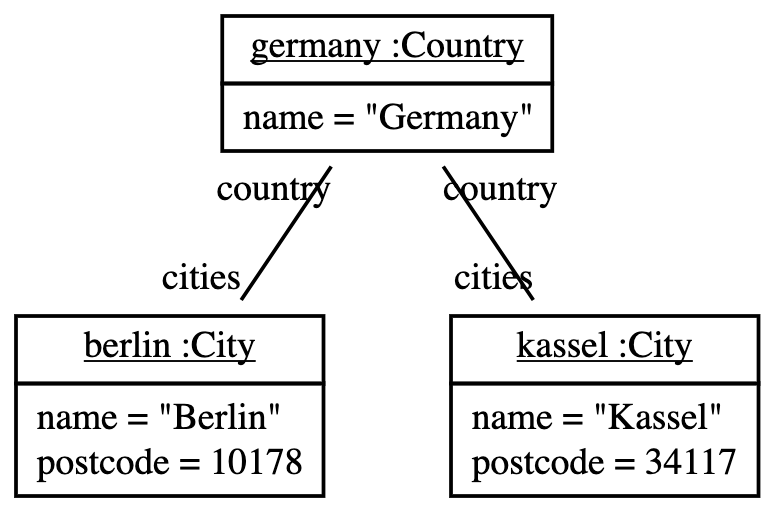
\includegraphics[width=0.5\textwidth]{chapter/fulib-scenarios/img/germany.png}
    \caption{Objektdiagramm von \code{Germany}}
    \label{fig:germany.png}
\end{figure}

Neben der Dateiendung \code{.png} wird auch \code{.svg} für Vektorgrafiken unterstützt.
Diese werden zwar vergrößert besser dargestellt, eignen sich aber u.U.\ nicht für die Einbettung in Markdown.
Des Weiteren existieren diverse weitere Ausgabeformate, welche in der Dokumentation~\cite[Language.Sentences.Test Sentences.Diagram Sentences]{documentation} näher erläutert werden.

\subsection{Kontrollstrukturen}\label{subsec:control-structures}

Mit Scenarios lassen sich nicht nur statische Objektstrukturen erzeugen.
Es ist auch möglich, zur Laufzeit Entscheidungen zu fällen und davon abhängig unterschiedliche Ergebnisse zu erzeugen.
Dafür kommen \code{As}-Sätze zum Einsatz.
Diese entsprechen If-Anweisungen in Java, jedoch mit dem konzeptuellen Unterschied,
dass im Scenario vom Eintreten der Bedingung ausgegangen wird.
Daraus folgt sowohl die Verwendung des Schlüsselworts \code{As} statt \code{If},
als auch die fehlende Syntax für \code{else}-Zweige\footnote{
Dies lässt sich durch Verwenden von zwei \code{As}-Sätzen mit gegensätzlichen Bedingungen umgehen.
}.

Das folgende Beispiel soll zur Illustration dieser Sätze dienen:

\begin{codeblock}
    As semester of Alice is less than 3, we add Maths to courses of Alice.
\end{codeblock}

Der \code{As}-Satz nimmt hier die Form \code{As <condition>, <sentence>.} an.
In der Bedingung wird der Wert des Attributs \code{semester} des Objekts \code{Alice} mit \code{3} verglichen, wobei \code{is less than} gleichzusetzen ist mit \code{<}.
Die Scenario-Sprache definiert Operatoren für Gleichheit (\code{is}), Ungleichheit (\code{is not}), Größer/Kleiner Als (\code{is greater/less than}) und Größer/Kleiner Gleich (\code{is greater/less equal}).

Ist die Bedingung wahr, wird der nachstehende Satz ausgeführt.
In diesem Beispiel ist dies ein \code{Add}-Satz, der Zahlen addieren und Elemente zu Listen bzw.\ Zu-n-Assoziationen hinzufügen kann.
In diesem Fall sind \code{Maths} und \code{Alice} im Vorhinein deklarierte Objekte;
\code{courses} ist eine Zu-n-Assoziation von der Klasse von \code{Alice} zu der Klasse von \code{Maths}.

Der zum obigen Beispiel gehörende Java-Code ist:

\begin{jcodeblock}
    if (alice.getSemester() < 3) {
        alice.withCourses(maths);
    }
\end{jcodeblock}

Um mehrere Sätze im Rumpf der If-Anweisung zu erhalten, können mehrere Sätze hinter dem \code{As}-Satz durch \code{and} getrennt werden:

\begin{codeblock}
    As Alice has done Maths, we add 6 to credits of Alice
    and we remove 3 from motivation of Alice.
\end{codeblock}

\begin{jcodeblock}
    if (alice.getDone().contains(maths)) {
        alice.setCredits(alice.getCredits() + 6);
        alice.setMotivation(alice.getMotivation() - 3);
    }
\end{jcodeblock}

Die zweite Art von Kontrollstruktur in der Scenario-Sprache ist der \code{Take}-Satz, der auf \code{for}-Schleifen in Java abgebildet wird.
Dieser nimmt die Form \code{We take a <name> from <expr> and <sentence...>} an, wobei \code{<name>} den Namen der Schleifenvariable, \code{<expr>} die zu durchlaufende Liste und \code{<sentence...>} den Schleifenrumpf bilden.
Im folgenden Beispiel ist diese Form ersichtlich:

\begin{codeblock}
    We take a student from students of uni and we add 1 to the semester of student.
\end{codeblock}

Übersetzt in Java-Code ergibt sich die \code{for}-Schleife:

\begin{jcodeblock}
    for (Student student : uni.getStudents()) {
        student.setSemester(student.getSemester() + 1);
    }
\end{jcodeblock}

Wichtig bei der Verwendung von \code{take} ist, dass der Ausdruck nach \code{from} einen \emph{Listentyp} hat.
Diese entsprechen in Java dem Typ \jcode{java.util.List<T>}, wobei \code{T} der Elementtyp ist.
Der Getter von Zu-n-Assoziationen hat automatisch einen Listentyp mit der Zielklasse als Elementtyp.

Es ist jedoch auch möglich, Listenausdrücke zu verwenden.
Diese bestehen in der einfachsten Form aus anderen Ausdrücken, die durch Komma oder \code{and} getrennt sind.
Beispiele dafür sind \code{1, 2, 3}, \code{Alice, Bob and Charlie} und \code{'left' and 'right'}.
In Java werden daraus Ausdrücke wie \code{Arrays.asList(1, 2, 3)} vom Typ \code{List<Integer>}.
Diese Listen lassen sich beispielsweise mit \code{write}-Sätzen in einer Variable speichern:

\begin{codeblock}
    We write Alice, Bob and Charlie into students.
\end{codeblock}

Daraus entsteht der folgende Java-Code:

\begin{jcodeblock}
    List<Student> students = new ArrayList<>(Arrays.asList(alice, bob, charlie));
\end{jcodeblock}

Zu beachten ist hier die Verwendung von \code{ArrayList};
durch diese können der Liste Elemente hinzugefügt oder entfernt werden.
Dies ist mit den \code{add}- und \code{remove}-Schlüsselwörtern möglich:

\begin{codeblock}
    We add David to students.
    We remove Bob and Charlie from students.
\end{codeblock}

\begin{jcodeblock}
    students.add(david);
    students.removeAll(bob, charlie);
\end{jcodeblock}

Listen haben in der Scenario-Sprache eine große Bedeutung, weshalb weitere Sprachfeatures deren Gebrauch vereinfachen.
Aus Platzgründen sind diese hier nicht weiter erläutert,
sie sind jedoch in der Dokumentation unter~\cite[Language.Expressions.Collections]{documentation} zu finden.

\subsection{Methoden}\label{subsec:methods}

Bisher wurde sämtlicher Code von Sätzen in Testmethoden generiert.
Die Scenario-Sprache sieht es aber auch vor, Aktionen auf Objekten durchzuführen, welche in Methoden gekapselt werden.
Dafür soll neben der Syntax für Methodenaufrufe auch die Zuordnung über Subjekte betrachtet werden.

Ein Methodenaufruf in der Scenario-Sprache beginnt stets mit einem \code{Call}-Satz.
Dieser nimmt die Form \code{We call <name> on <receiver> with <parameters...>} an, wobei sowohl Empfänger als auch Parameter optional sind.
Ein einfaches Beispiel ist folglich:

\begin{codeblock}
    We call init.
\end{codeblock}

Da sich \code{we} auf den Test bezieht und es keinen Empfänger gibt, ist das Testobjekt der Empfänger.
In der Testklasse wird eine Methode \code{init} angelegt, die an der Stelle des Satzes aufgerufen wird:

\begin{jcodeblock}
    init();
    // ...
    void init() {
    }
\end{jcodeblock}

Nach dem \code{Call}-Satz folgt der Rumpf.
Da es in der Scenario-Sprache keine geschweiften Klammern o.ä.\ gibt,
muss auf andere Weise zwischen den Sätzen unterschieden werden, die zum Rumpf gehören,
und jeden, die in der Testmethode auf den Aufruf folgen sollen.
Dafür dienen die Subjekte jedes Satzes.
Bei den meisten bisher kennengelernten Sätzen war dies \code{We}, welches sich stets auf die Testmethode bezieht.
Viele Sätze erlauben jedoch alternativ die Angabe eines Methodennamens wie \code{init} aus dem obigen Beispiel.
So kann festgelegt werden, dass sie zum Rumpf eines vorherigen Aufrufs gehören.
Die \code{init}-Methode kann also wie folgt gefüllt werden:

\begin{codeblock}
    We call init.
    Init writes ... into students.
    Init takes a student from students and init adds ... .
\end{codeblock}

Zu beachten ist, dass einige Sätze wie \code{expect} oder Diagramme nur in Tests erlaubt sind.
Bei anderen Sätzen wie \code{is} und \code{has} hat das Subjekt eine andere Bedeutung,
wodurch sie automatisch zum aktuell beschriebenen Rumpf oder Test gehören.
Zudam lassen sich Subjekte nicht mischen;
verwendet ein Satz ein anderes Subjekt als der vorherige, wird der vorherige Aufruf geschlossen.
Hat ein \code{call}-Satz ein anderes Subjekt als \code{we}, können geschachtelte Methodenaufrufe stattfinden.
Dadurch lässt sich u.A.\ Rekursion realisieren.
Der geschachtelte Aufruf kann zwar wieder einen neuen Rumpf beginnen, davon ist jedoch aus Gründen der Verständlichkeit abzuraten.

Während eine \code{init}-Methode für gemeinsam genutzen Code in einem Test akzeptabel ist,
sollten Methoden mit Business Logic üblicherweise nicht in Tests implementiert sein.
Dabei kommt der Empfänger bei \code{call}-Sätzen zum Einsatz.
Dieser wird zum Empfänger des Aufrufs in Java, und die Methode wird Teil dessen Klasse, wie das folgende Beispiel zeigt.

\begin{codeblock}
    We call do-work on Alice.
    Do-work removes 1 from the motivation of Alice.
\end{codeblock}

\begin{jcodeblock}
    alice.doWork();

    class Student {
        // ...
        void doWork() {
            this.setMotivation(this.getMotivation() - 1);
        }
    }
\end{jcodeblock}

Hier ist auffällig, dass im zweiten Satz, der den Rumpf der Methode bildet,
aus der Referenz zu \code{Alice} das Schlüsselwort \code{this} wird.
Dies ist eine Konsequenz dessen, dass innerhalb des Rumpfes die Variablen des Tests nicht mehr zugänglich sind.
Ausnahme ist dabei der Empfänger des Aufrufs, der mit \code{this} zugänglich ist.

Ein ähnliches Verhalten ist beim Verwenden von Parametern zu beachten.
Dieses Beispiel zeigt einen Aufruf mit einem solchen:

\begin{codeblock}
    We call give-assignment on Alice with assignment a1.
    Give-assignment adds a1 to todo of alice.
\end{codeblock}

Im Java-Code ist erkennbar, dass aus \code{a1} im Rumpf eine Referenz auf den \code{assignment}-Parameter wird:

\begin{jcodeblock}
    alice.giveAssignment(a1);

    class Student {
        // ...
        void giveAssignment(Assignment assignment) {
            this.withTodo(assignment);
        }
    }
\end{jcodeblock}

Mehrere Parameter werden wie üblich durch \code{and} und Kommata getrennt.
Diese sind zwar benannt, müssen aber dennoch bei jedem Aufruf in der gleich Reihenfolge stehen.

Die bisher gezeigten Beispiele für Methoden zeichneten sich durch ihren Gebrauch von Seiteneffekten aus.
Dies ist nicht immer gewünscht und u.U.\ hinderlich, weshalb die Scenario-Sprache auch Syntax für Rückgabewerte bereitstellt.
Dies erfolgt durch \code{Answer}-Sätze, welche \code{return}-Anweisungen in Java entsprechen.

\begin{codeblock}
    We call produce on factory.
    Produce creates a product.
    Produce answers with the product.
\end{codeblock}

Diese Beispiel verwendet den \code{Create}-Satz, der semantisch einem \code{There}-Satz entspricht, aber durch die Präsenz eines Subjekts in Methoden Anwendung findet.
Am Java-Code ist zu erkennen, dass durch die Verwendung eines benannten Objekts als Rückgabewert auch beim Aufruf eine Variable erzeugt wird:

\begin{jcodeblock}
    Product product = factory.produce();

    class Factory {
        // ...
        Product produce() {
            Product product = new Product();
            return product;
        }
    }
\end{jcodeblock}

Wird diese Methode erneut aufgerufen, darf der Rumpf nicht erneut wiederholt werden.
Somit ist auch kein Variablenname für das Ergebnis angegeben.
Ohne diesen kann jedoch nicht nach dem Aufruf darauf zugegriffen werden.
Aus diesem Grund existiert der \code{answer}-Ausdruck, mit dem auf das letzte Ergebnis eines Methodenaufrufs zugegriffen werden kann.
Das folgende Beispiel illustriert dessen Verwendung:

\begin{codeblock}
    We call produce on factory.
    We add the answer to payload of transporter.
\end{codeblock}

\begin{jcodeblock}
    Product result1 = factory.produce();
    transporter.withPayload(result1);
\end{jcodeblock}

Hier wird das Ergebnis des Aufrufs in der automatisch benannten Variable \code{result1} gespeichert.
Aus \code{the answer} wird dann im Java-Code ein Zugriff darauf.

Zuletzt soll das Konzept der \emph{Stückweisen Definition}, welches bei Methoden Anwendung findet, betrachtet werden.
Dieses erlaubt es, bei jedem Aufruf einer Methode einen Teil ihres Rumpfes zu definieren.
Der Compiler fügt diese Teile hintereinander, um den ganzen Rumpf der Methode zu bilden.
Dazu soll nun ein vollständiges Beispiel betrachtet werden.
Ziel ist es, eine Benutzerdatenbank zu modellieren, in der Benutzer mit IDs abgelegt sind.
Diese definiert eine Operation \code{getOrCreate}, die gegeben eine ID entweder einen existierenden Benutzer mit dieser ID findet,
oder einen neuen anlegt und speichert.
Listing~\ref{lst:UserRegistry.md} zeigt das entsprechende Scenario.

\codelisting{md}{chapter/fulib-scenarios/scenarios}{UserRegistry.md}{Beispielscenario für Benutzerdatenbank mit stückweiser Definition}

Dabei wird zunächst unter \code{Setup} das Datenmodell definiert.
Dazu gehören die Klassen \code{User} und \code{UserRegistry},
die über eine Assoziation miteinander verknüpft sind.
\code{User} hat ein Attribut \code{id} vom Typ \code{int}.
Von beiden Klassen wird jeweils ein Objekt angelegt.

Unter \code{Get Existing} folgt der erste Aufruf der Methode \code{getOrCreate} in \code{UserRegistry},
wobei eine ID als Parameter übergeben wird.
Dabei wird mit einer Schleife nach einem bereits existierenden, mit der Registry verknüpftem \code{User} mit dieser ID gesucht.
Da unter \code{Setup} bereits ein solcher angelegt wurde, ist die Suche erfolgreich und endet mit der Rückgabe dessen.
Daraufhin wird mit einem \code{Expect}-Satz geprüft, ob auch wirklich das richtige Objekt zurückgegeben wurde.

Unter \code{Create New} folgt der zweite Aufruf der Methode.
Hier soll ein neues \code{User}-Objekt angelegt werden.
Deshalb beschreibt das Scenario an dieser Stelle, wie die \code{getOrCreate}-Methode dies durchführen soll (durch Erzeugen eines Objekts und Erstellen einer Verknüpfung mit der Registry).
Das neue Objekt wird daraufhin zurückgegeben und erneut durch den Test geprüft.

Betrachtet man nun den generierten Java-Code für die \code{UserRegistry}-Klasse,
wird deutlich, wie die beiden Teildefinitionen des Methodenrumpfes zusammengefügt wurden.
In Listing~\ref{lst:UserRegistry_getOrCreate.java} ist dies an \code{(1)} und \code{(2)} sichtbar.

\codelisting{java}{chapter/fulib-scenarios/java}{UserRegistry_getOrCreate.java}{\code{UserRegistry.getOrCreate}-Methode}

Der aus dem Scenario generierte Test sowie die vollständigen \code{User}- und \code{UserRegistry}-Klassen sind in Anhang~\ref{sec:user-registry-full} zu finden.
